\chapter{Radar system overview}

In order to build a model capable of accurately capturing key features from target surfaces one must first understand the origin of the received signal. In this chapter a few fundamental concepts in radar systems are introduced that explain how range, velocity and reflectivity arise in a \gls{pcr} system. The mixing and IQ demodulation procedures are also discussed, which explain how a returning radar echo is captured and demodulated. 

\section{Target properties from radar response}
% TODO: Utilize https://acconeer.sharepoint.com/:w:/g/CS/ES_xwcoTqVdGkShPJkNagMMBL1wVd_GaeJJsEDKC8lWIDQ?e=GxZNEw as a source for this.
Fundamentally, a radar operates by radiating \gls{rf} electromagnetic energy and listening if the transmitted energy generates any echoes \citep{skolnik_2009}. By analyzing properties of the returning signal it is then possible to obtain information about the target objects that scattered the transmitted pulse. This may involve the distance and angle at which scatterers are located or which velocity they are moving in. With a sufficiently high angular and range resolution it is even possible to descern parts of the targets' sizes and shapes.  

Radars are typically active systems, meaning that they have a radiating antenna and do not depend on ambient radiation \citep{richards_2014}. Radar measurements can be performed in a number of ways. In this report a \gls{pcr} system is used. This means that a sequence of short wavelets are transmitted towards a target scene to determine its properties. One such transmitted wavelet pulse $x_T(t)$ has some carrier frequency $f_t$ and envelope $A(t)$ as in

\begin{equation}\label{eq:trans}
	x_T(t)
	= A(t)\sin(2\pi f_t).
\end{equation}

After various scattering processes, the returning signal is analyzed. This can be done either using an one or two dimensional array of antennas or just using a single antenna. 

\subsection{Single-antenna considerations}

Commonly, in larger radar systems, many receiving antennas capture the returning radiation. This allows for distinguishing radar targets not only in range, but also allows for the radar to have angular resolution. In this work a single receiving antenna is used, meaning that the radar has no intrinsic method of determining at which angle a scatterer is located, obtaining snapshots of the entire scene. Hence, the sensor used in this work is only capable of acquiring one-dimensional signals. 

To understand what information can be obtained from such a one dimensional signal, a single scattering object some distance away from the transmitter is here considered. If a radar pulse with envelope $A(t)$ and frequency $f_t$ is transmitted towards it, the returning signal will be on the form \citep{richards_2014}

\begin{equation}\label{eq:returning}
	r(t) = CA(t-D)\sin(2\pi f_t (t-D))
\end{equation}

where $D$ is some delay and $C$ a constant related to the dissapation of power throughout space and some radar system properties. For the purposes of this report, the properties of the phase shift $\phi=-2\pi f_tD$ is of particular interest. In the next two sections, it is shown how distance and velocity can be deduced from this parameter using the time delay and the Doppler shift. The $C$ variable carries information too, described lastly. 

\subsection{Radar distance measurements}

If a scatterer was present a distance $d$ from the transmitting antenna, a wavelet will return $2d/c$ seconds after transmission, where $c$ denotes the speed of light. The 2 appears to accomodate for the pulse traveling back and forth (or, perhaps more accurately, forth and back) between the sensor and the scatterer. Hence, the transmitted signal is delayed according to 

\begin{equation}
	\begin{split}
		r(t) 
		& = CA(t-2d/c)\sin(2\pi f_t(t - \frac{2d}{c})) \\
		& = CA(t-2d/c)\sin(2\pi f_tt - \frac{4\pi d}{c}f_t).
	\end{split}
\end{equation}

where the phase shift $\phi$ is equal to $-4\pi f_t d/c$. If we can find $\phi$, the distance can then be calculated through

\begin{equation}
	d
	= \frac{c \phi}{4\pi f_t}
	= \frac{\phi}{4\pi}\lambda.
\end{equation}

Thus, by examining the shift in phase of the returning signal, we can deduce the distance to the scattering object. 

\subsection{Doppler frequency in pulsed radar}
\label{doppler}

If the target scatterer is moving from or towards the transmitting antenna, a frequency shift will occurr. For velocity $v$, the transmitted frequency $f_t$ will be shifted to $f_r$ according to the well known Doppler formula \citep{ridenour_1947}

\begin{equation}
	f_r = \frac{c + v}{c - v}f_t
\end{equation}

where positive $v$ indicates that the scatterer is moving towards the transmitter. The frequency shift $f_d$, also known as the \emph{beat frequency} \gls{bf}, is then

\begin{equation}\label{eq:dshift}
	f_d 
	= f_r - f_t 
	= \frac{2v}{c-v}f_t \approx \frac{2v}{c}f_t 
	= \frac{2v}{\lambda_t}.
\end{equation}

This shift means that the an approaching target has slightly increased returning frequency, and conversely that a receeding target has a slightly decreased frequency. In this project a pulsed radar is used, meaning that measurements are done repeatedly using short wavelets instead of transmitting one continuous wave. What does this mean for the Doppler shift?

For a pulsed radar system, with sampling frequency $F_s$ and sampling period $T_s = 1/F_s$, the Doppler shift can be viewed as a phase shift from one pulse to the next. Between two pulses, a target moves a distance $vT_s$. Hence, each pulse travels a distance $2vT_s$ less than the preceding one. This distance corresponds to $2vT_s/\lambda_t$ wavelengths, providing a phase change per pulse of

\begin{equation}
	\Delta \phi = \frac{4\pi}{\lambda_t}vT_s.
\end{equation}

For a target moving at a constant pace, the beat frequency arising from the constant doppler phase shift is thus $f_d = 2v/\lambda_t$, as was found in equation \ref{eq:dshift}. 


\subsection{Power dissapation}

The $C$ factor in \ref{eq:returning} describes the ratio of the emitted power that is returned after a scattering process has occurred. Assuming that the trasmit power $P_t$ is radiated isotropically by a point source, the power density distributed uniformly by the source over the surfase of a sphere of radius $R$ is \citep{amin_2017}

\begin{equation}
	P_d 
	= \frac{P_t}{4\pi R^2}.
\end{equation}

If a scatterer is present at range $d$ with radar cross section $\sigma$ and gain $G_t$, the fraction of the radar power reflected by the target is given by 

\begin{equation}
	P_{e}
	= \frac{P_tG_t\sigma}{4\pi d^2}.
\end{equation}

Then, given that the scattering process is isotropic, the power reflected back at the radar receiver is

\begin{equation}\label{eq:temp}
	P_f 
	= \frac{P_e}{4\pi R^2} 
	= \frac{P_t G_t \sigma}{(4\pi d^2)^2}.
\end{equation}

Finally only a portion $P_r = P_eA_r$ of the power is captured by the receiver, where $A_r$ is a function of transmission wavelength and receive antenna gain. Including this into \ref{eq:temp}, we obtain the \emph{radar range equation} relating the transmitted and recieved power as

\begin{equation}
	P_r
	= \frac{P_t G_t A_r \sigma}{16\pi^2 d^4}.
\end{equation}

The radar range equation states that power dissapates rapidly, by a factor $1/d^4$, with range. Thus, increasing the distance to a target object with a factor 2 will return only $1/16$ of the power otherwise received. If the noise power $N$ remains constant regardless of target distance, the \emph{signal-to-noise ratio} (\gls{snr}), defined as $\text{SNR} = P_r/N$ quickly decreases with range. 

We also see from the radar range equation that the power returned is also governed by the \emph{radar cross section} (RCS) $\sigma$ of the target. This ascribed area is the projected area of a metal sphere which would return the same echo at hand had the sphere been substituted for the target \citep{skolnik_2009}, and is used for quantifying the echo in terms of reflectivity.  

% Have a part on bandwidth




%\section{Radar operation}

%A pulsed radar system can be realized in countless ways, but all subscribe to the fundamental physical laws of electromagnetic radiation. In this section one such configuration is described. Furthermore, we describe the key signal processing method, \emph{In-phase and Quadrature-phase demodulation} (IQ demodulation), used for extracting useful information from the unprocessed radar response. 

%\subsection{Elements of a pulsed radar}
%The radar system considered in this report includes the following crucial components:

%\begin{itemize}
%	\item Waveform generator
%	\item Oscillator
%	\item Transmitting antenna
%	\item Receiving antenna
%	\item Mixer
%	\item Integrator
%\end{itemize}

% List of parts in radar system
% Nice figure showing this process


%A waveform generator outputs a radar envelope which is modulated by a local oscillator to some desired radio frequency. After signal amplification the wavelet is transmitted through an antenna. Detection is performed by a second antenna, which receives the returning signal during some time interval. 

\section{Mixing}

In the preceding section it was shown that the scattering response carry information about target range, reflectivity and velocity from or towards the sensor. This section explains how the radar captures the returning signals to generate raw radar data, shown in fiugre \ref{fig:single_sweep_raw} through a process known as \emph{mixing}.

An incoming signal from a single scattering point target is on the form described in \ref{eq:returning}. Mixing involves generating an internal pulse, called an analysis pulse, of equal frequency of what was transmitted. The captured signal and the generated signal are then multiplied elementwise and summed, to form one measurement $m(\tau)$, where $\tau$ is the internal delay of the analysis pulse. The mixing process is illustrated in figures \ref{fig:mix0} and \ref{fig:mix1}. The analysis pulse is shown in the top plot, the recieved pulse in the center plot and the result of the elementwise multiplication is shown at the bottom. These two figures differ in that the internal delay $\tau$ of the analysis pulse are different, so that no overlap occurrs in the first figure while significant overlap happens in the second. 

Mathematically we can describe this procedure as

\begin{equation}
	m(\tau) = \int_{-\infty}^{+\infty} x_T(t - \tau)r(t) dt
\end{equation}

where $x_T(t)$ and $r(t)$ are the transmitted and received pulses respectively, as defined in \ref{eq:trans} and \ref{eq:returning}. If only a single point scatterer is in the target scene and $A(t)$ is a rectangular window of length $L$

\begin{equation}
	A(t) = \begin{cases}
		1 & \text{if $0\leq t < L$} \\
		0 & \text{otherwise},
	\end{cases}
\end{equation}
then $m(\tau)$ will be on the form 

\begin{equation}
	m(\tau) = 
	\begin{cases}
		0 & \text{if $|\tau-2d/c|\geq L$} \\
		\text{(\ref{eq:n1})} & \text{if $|\tau-2d/c|<L$ and $\tau \leq 2d/c$} \\
		\text{(\ref{eq:n2})} & \text{if $|\tau-2d/c|<L$ and $\tau > 2d/c$}
	\end{cases}
\end{equation}

\begin{equation}\label{eq:n1}
	\frac{C}{2}\Big((\tau + L - D)\cos(2\pi f_t(\tau - D)) 
	- \frac{1}{2\pi f_t}\sin(2\pi f_t(\tau - D))\Big)
\end{equation}

\begin{equation}\label{eq:n2}
	\frac{C}{2}\Big((D + L - \tau)\cos(2\pi f_t(\tau - D)) 
	+ \frac{1}{2\pi f_t}\sin(2\pi f_t(\tau - D))\Big).
\end{equation}

The full derivation of \ref{eq:n1} and \ref{eq:n2} can be found in the appendix. In figure \ref{fig:mix2}, a numerical computation of the mixing procedure, shown in part in figures \ref{fig:mix0} and \ref{fig:mix1}, has been performed. Note that this result was obtained for a noise-free mixing of a signal from a single scattering target. It is thus clear that with complicated continuous structures, target scenes produce complex outputs at the reciever. 

In \ref{fig:single_sweep_raw}, a mixing output from the radar sensor used in this project is shown. For this example, the target scatterer is a hand held approximately 15 cm from the sensor. 



%In this work we are investigating moving targets, which renders doppler frequency shifts in the echo waveform. Thus we are primarily interested in detecting veclocity components in $r(t)$, which shows up in the $\theta(t)$ function. Effective tracking of the $\theta(t)$ function can be achieved through \emph{IQ demodulation}. 


%Our target is to find $\theta(t)$, providing information about the target scatterer.  




%We previously stated that after the radar has transmitted a pulse, it listens for an echo. This process is more formally called \textit{mixing}. After having transmitted a pulse, an internal wavelet is generated at a very specific delay from the initial pulse transmission. This internal wavelet is multiplied with the received signal. If the received and internal pulses do not match, the output of this multiplication will be zero. If there however exist some overlap between the internal and returning signals the output will be nonzero, indicating some level of energy content at the distance corresponding to the internal pulse delay. By increasing the internal pulse delay and repeating this procedure a set of measurement points is obtained. Mixing is thus achieved by multiplying a large number of returning wavelets with internally generated wavelet counterparts, adding a slight delay between sampling points. 

% Describe why this process is equivalent to an autocorrelation
% Include plot of raw data to show what a real sweep looks like.

%Figures \ref{fig:mix0}, \ref{fig:mix1} and \ref{fig:mix2} illustrate this principle. In the upper plot in the first two figures two analysis wavelets are shown, each at a different time delay. The center plot show the received radar pulse registrered by the antenna, and the lower plot the result when the two above signals are multiplied elementwise. Note that the final figure show the result of multiple received electromagnetic pulses, each sample point representing a summation of one set of multiplications between returning and internally generated signals. This output will henceforth be called the \emph{raw signal}.   

\begin{figure}[h]
	\centering
	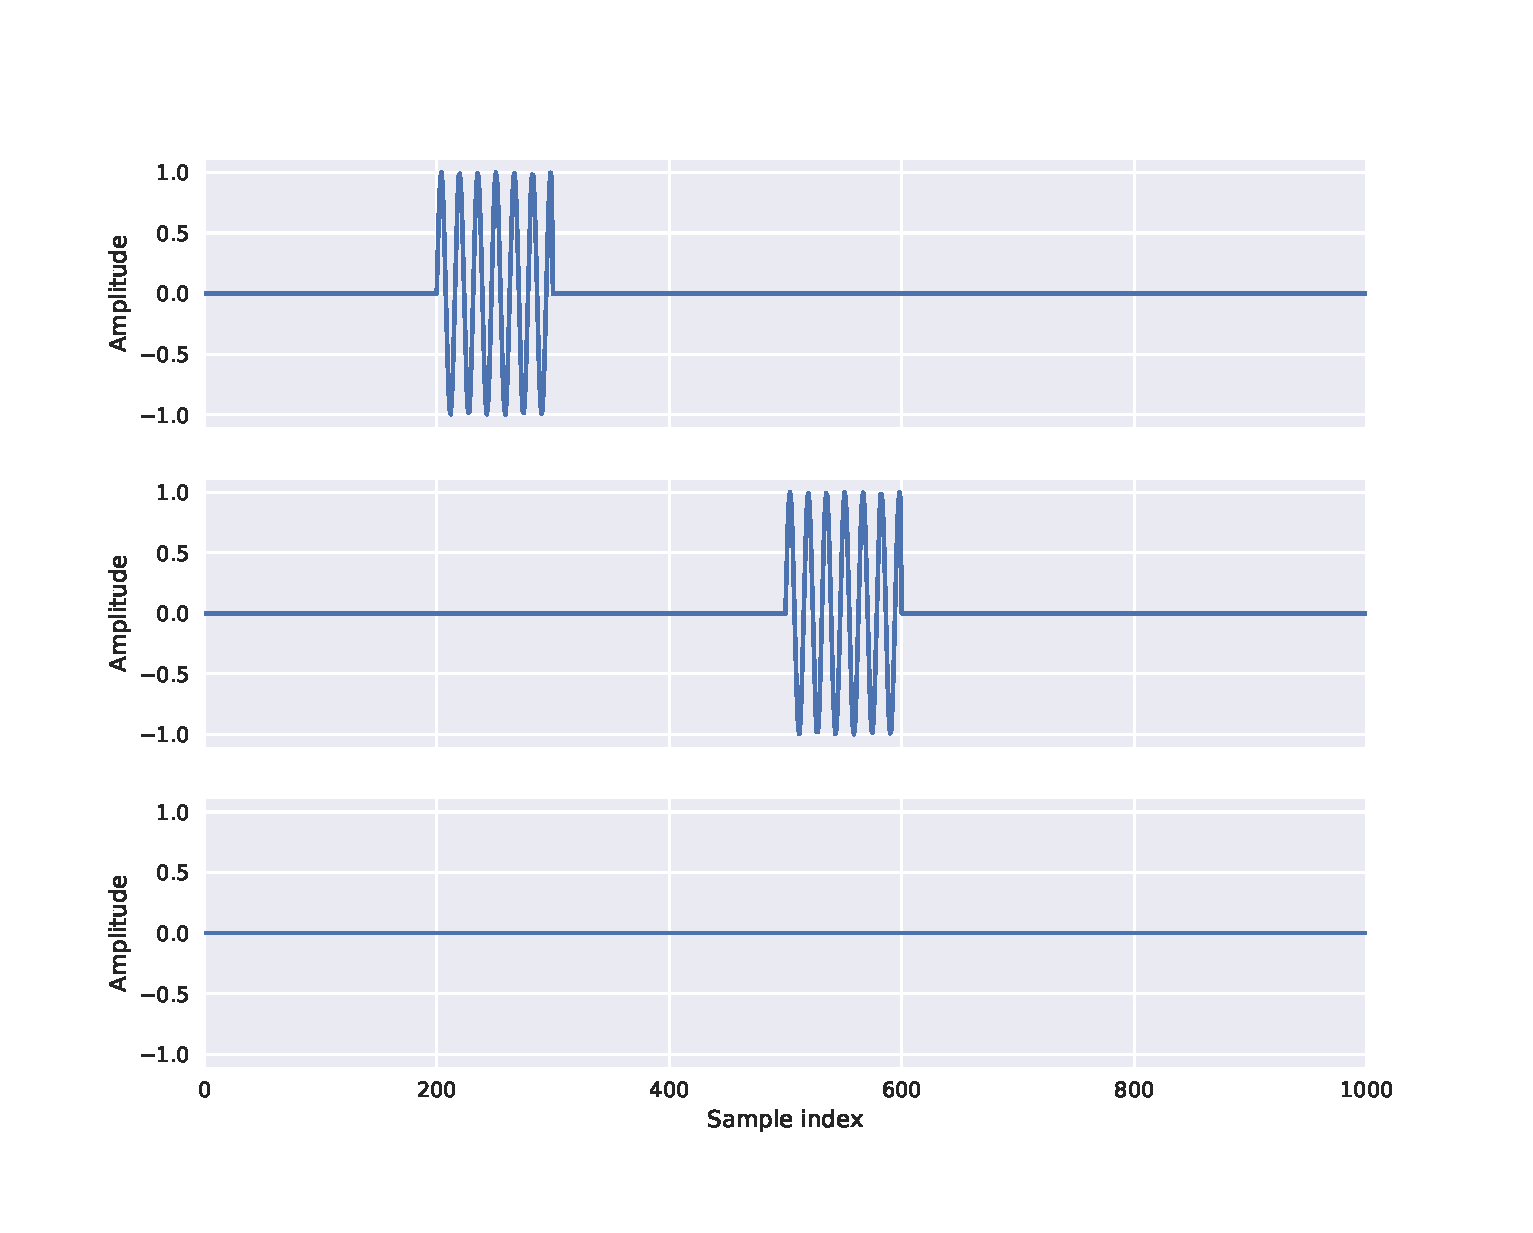
\includegraphics[scale=0.5]{figs_temp/mixing0}
	\caption{Analysis pulse (top), received pulse (mid) and multiplication output (bot). As the signals do not overlap the multiplication yields only zero values.}
	\label{fig:mix0}
\end{figure}

\begin{figure}[h]
	\centering
	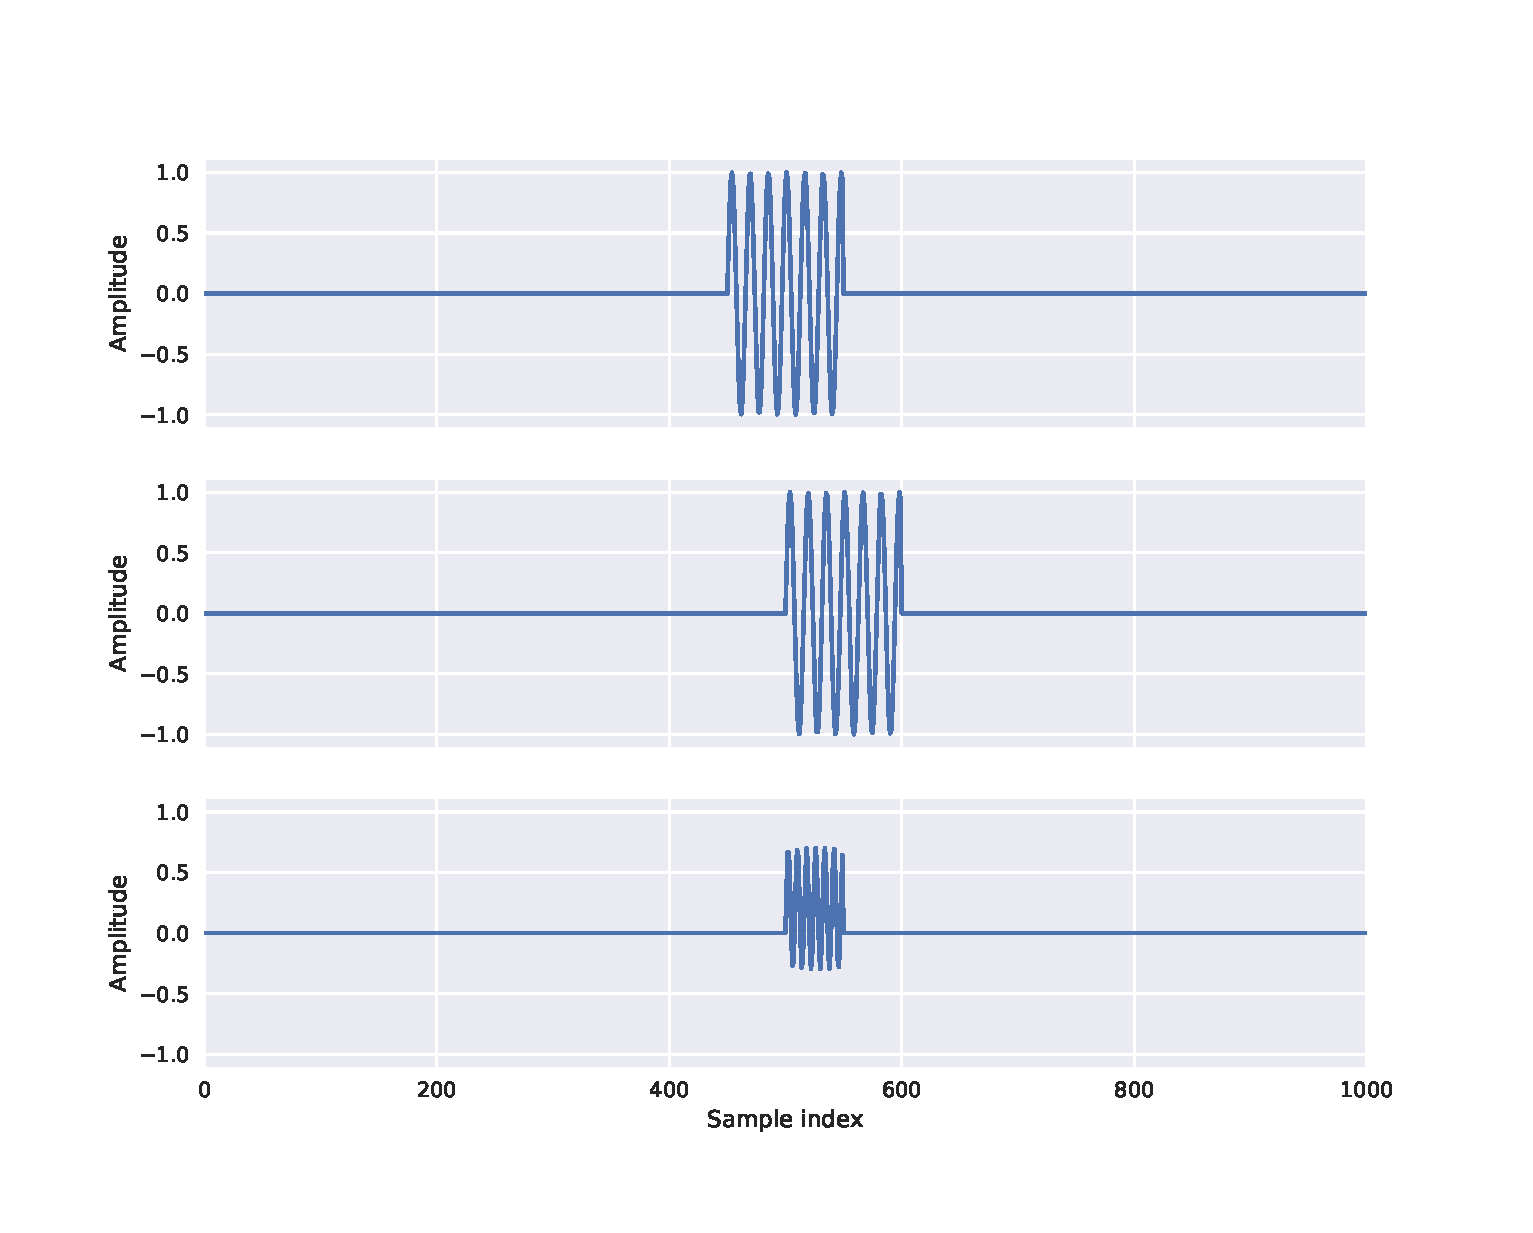
\includegraphics[scale=0.5]{figs_temp/mixing1}
	\caption{Analysis pulse (top), received pulse (mid) and multiplication output (bot). The overlapping signals produce varying amplitudes at the output sensitive to small changes in phase.}
	\label{fig:mix1}
\end{figure}

\begin{figure}[h]
	\centering
	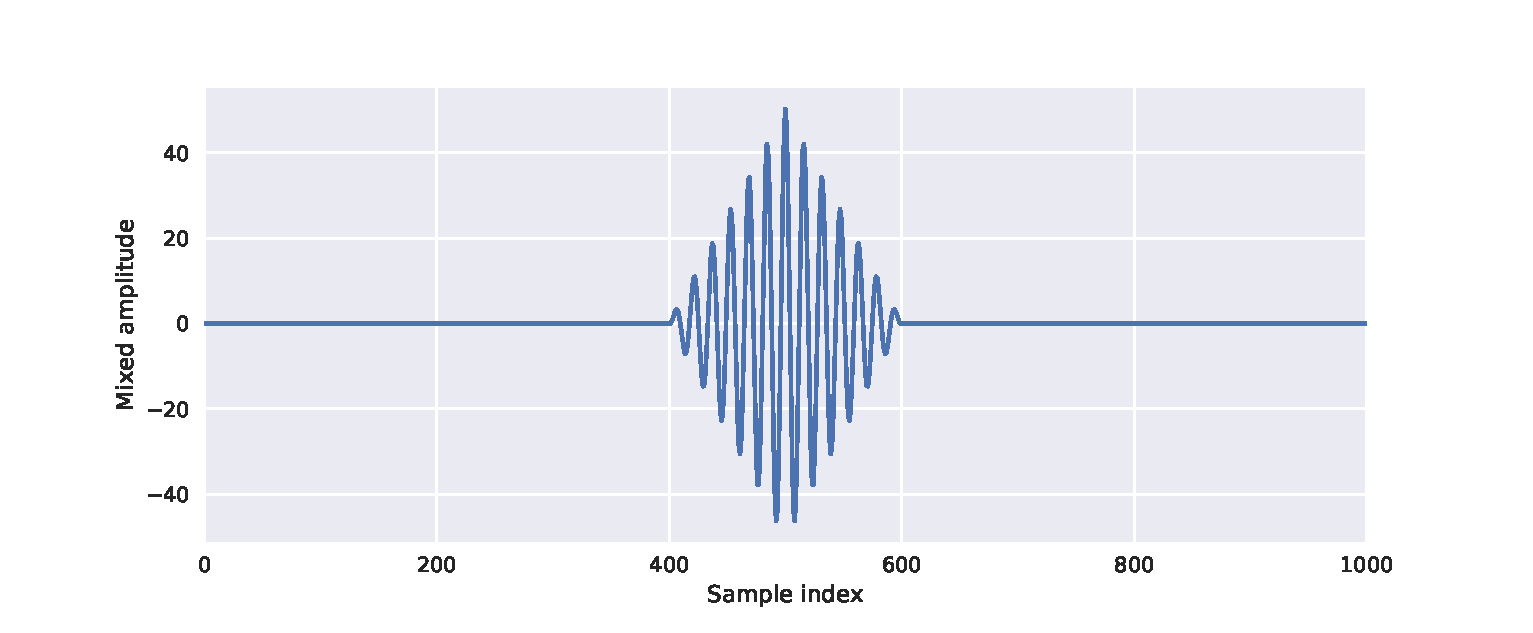
\includegraphics[scale=0.5]{figs_temp/mixing2}
	\caption{By integrating the multiplication at each delay the mixing output is produced.}
	\label{fig:mix2}
\end{figure}

\begin{figure}[h]
	\centering
	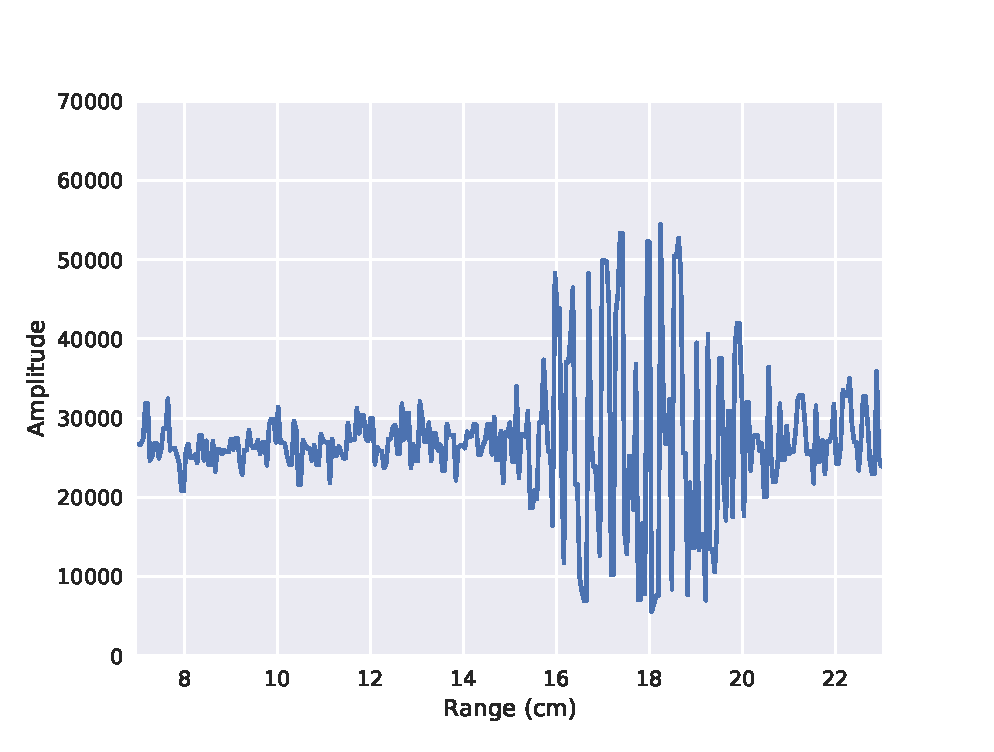
\includegraphics[scale=0.7]{figs_temp/single_sweep_raw}
	\caption{A single radar sweep which has been measured from 7 to 23 cm. The largest amplitude at around 18 cm. suggests there is some object present at that distance from the sensor.}
	\label{fig:single_sweep_raw}
\end{figure}

\section{IQ demodulation}
\label{IQ}

Even though single-antenna systems have no angular resolution, it was shown above that the returning signal carries useful information. By measuring the temporal shift from transmission to reception, we can calculate the distance to a scatterer, and by examining the phase shift between pulses, we may find the \gls{bf} and thus the radial velocity of the scatterer. Finally, the scatterers dielectric properties are brought forward through the \gls{rcs}, showing up as a scaling factor in the mixing output.

Although the raw signal produced by mixing shown in \ref{fig:single_sweep_raw} holds the information we are interested in, it has low \gls{snr} and is commonly avoided \citep{richards_2014}. Instead, some transformation of the raw signal is usually performed. In this work we are particularly interested in resolving small Doppler shifts, and thus we wish to closely monitor phase shifts from one measurement to the next. One effective method focusing on accurate phase tracking involves splitting the signal into its \emph{In-phase} and \emph{Quadrature} components, or IQ components. 

The in-phase channel mixes the raw signal with an oscillator at the radar frequency $f_t$, and the quadrature channel with the same frequency but with a $90^\circ$ phase shift from the I channel oscillator. After low-pass filtering, the IQ components are intepreted as a complex number

\begin{equation}
	x(t) = I(t) + jQ(t).
\end{equation}

IQ demodulation shifts the information bearing part of the mixed signal to baseband, meaning that an echo waveform on form $A(t)\sin(2\pi f t + \phi(t))$ after demodulation becomes $x(t) = A(t)e^{j\phi(t)}$.

The details of this demodulation scheme can be found in the appendix. In figure \ref{fig:single_sweep_iq} the amplitude $|x(t)|$ is shown for data captured using the same measurement setup as in figure \ref{fig:single_sweep_raw}. Although the amplitude may be useful, the real power of splitting the signal in I and Q components come from its phase tracking capabilities, as the phase is more sensitive to small changes in range than the amplitude \citep{lien_gillian_karagozler_amihood_schwesig_olson_raja_poupyrev_2016}.


% TODO: Incorporate more of what is written below. Intermediary frequency? Discuss with Peter. 


%A common type of data when working with radar signal processing is in-phase and quadrature-phase data (IQ-data). IQ-data is represented as complex numbers, and a radar sweep consists of several such complex numbers - one for each investigated range. The process of obtaining IQ-data is often referred to as IQ- or quadrature demodulation, and is described in appendix .... The usefulness of this type of data lies in that it contains explicit information about the amplitude, $A(t)$, and phase, $\theta(t)$, in equation \eqref{eq:raw_sweep} \citep{richards_2014}. To obtain the amplitude for a sweep, $s$, one simply computes the absolute value for each complex number in $s$. The amplitude plot is a good way to visualize at what ranges objects are present. Figure \ref{fig:single_sweep_iq} illustrates such a graph where the same measurement setup as in figure \ref{fig:single_sweep_raw} has been used. Similarly, a phase curve can be obtained by computing the phase in each point.

%In many applications, the phase information in IQ-data is used when small changes in the radar signal need to be detected, (Mention a case such as recording over grass...) as the phase is more sensitive to changes than the amplitude \citep{lien_gillian_karagozler_amihood_schwesig_olson_raja_poupyrev_2016}. If an object is detected at distance $r(t_1)$ from the radar at time $t_1$, and shortly thereafter, the object is moved to distance $r(t_2)$, the corresponding difference in phase will be
%\begin{equation}
%	\label{eq:phase_diff}
%	\Delta\phi(t_1, t_2)=\frac{4\pi}{\lambda}(r(t_2)-r(t_1)) \quad\quad \textrm{mod 2$\pi$}
%\end{equation}
%By having a sampling frequency which is too low, the range difference in $\eqref{eq:phase_diff}$ could potentially become very big, and the phase difference would fluctuate over time and be incomprehensible.

%In the case of material classification, a high sampling frequency is highly beneficial. When moving across surfaces characterized by tiny details, a high sampling frequency is essential in capturing the shapes of these.

\begin{figure}[h]
	\centering
	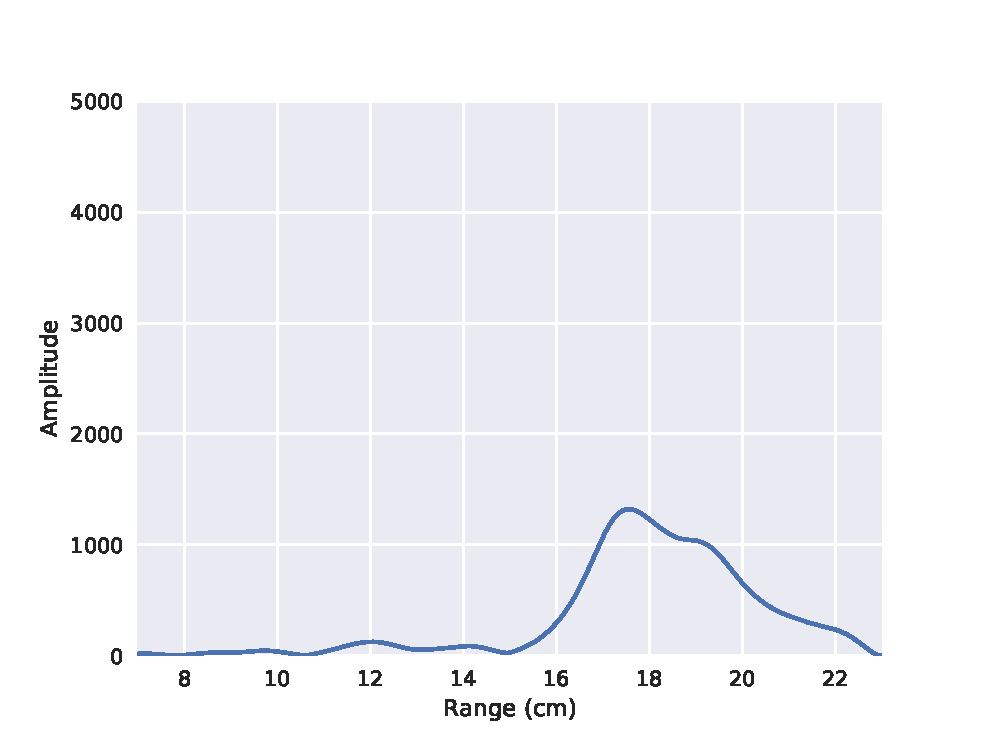
\includegraphics[scale=0.7]{figs_temp/single_sweep_iq}
	\caption{Visualization of an amplitude function derived from IQ-data.}
	\label{fig:single_sweep_iq}
\end{figure}

%For a thorough description of how IQ-data is derived, see appendix ...











%
%

